\documentclass[serif]{beamer}

\usetheme{CambridgeUS}
\usecolortheme{dolphin}

\usepackage{bm,color}
\usepackage{graphicx}
%\usepackage[brazil, english]{babel}
\usepackage{mathrsfs,amssymb,amsmath,enumerate}
%\usepackage{tgschola}
\usepackage{verbatim,graphicx,geometry,color}
\usepackage{caption, subcaption}
\usepackage[utf8]{inputenc}
%\usepackage{setspace}
\usepackage{amsthm}

\newtheorem{prop}{Proposition}
%\newtheorem{lemma}{Lemma}[section]
\theoremstyle{definition}


\newcommand{\E}{\mathbb{E}}
\newcommand{\Var}{\mathrm{Var}}
\newcommand{\plim}{\overset{p}{\longrightarrow}}
\newcommand{\dlim}{\overset{d}{\longrightarrow}}

\usepackage{hyperref}
%\hypersetup{
%  colorlinks = true,
%  linkcolor = red!60!black,
%}
%\renewcommand{\thefootnote}{\arabic{footnote}}
%
%\makeatletter
%\let\@mycite\@cite
%\def\@cite#1#2{{\hypersetup{linkcolor=blue!60!black}[{#1\if@tempswa , #2\fi}]}}
%\makeatother


\begin{document}

\title[Welfare Comparisons]{Welfare Comparisons for New Technology and New Combination Subsidies}
\author[Alexandre Sollaci]{Alexandre Sollaci}
\institute[UChicago]{The University of Chicago}
\date{\today}

\begin{frame}[noframenumbering]
\titlepage
\end{frame}

\frame{\frametitle{Summary}
\begin{itemize}
\item The figures show the welfare gains of a new technology subsidy and a new combinations subsidy for different subsidy values.
\item Each figure displays the same results but for a different period over which the subsidy is implemented and welfare is calulated -- e.g. introduce a subsidy for $X$ years and compute the welfare variation in those $X$ relative to the economy without any subsidy.
\item In the second part, I added figures that summarize what is happening in the economy when a subsidy is implemented. 
\item I use a 50\% subsidy as the example, since 50\% is the value (of a new combinations subsidy) that maximizes welfare when we look at the 15 year window.
\end{itemize}
}

\frame{\frametitle{5 years of subsidy}
\begin{figure}[h!]
\centering
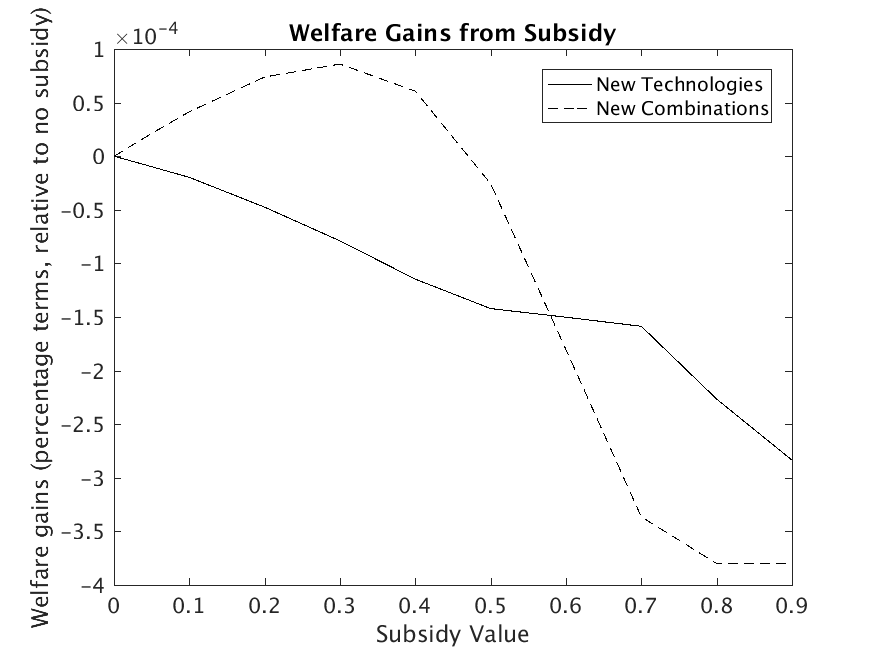
\includegraphics[width=.8\textwidth]{figures/5_years/welfare_gains.png}
\end{figure}
}

\frame{\frametitle{10 years of subsidy}
\begin{figure}[h!]
\centering
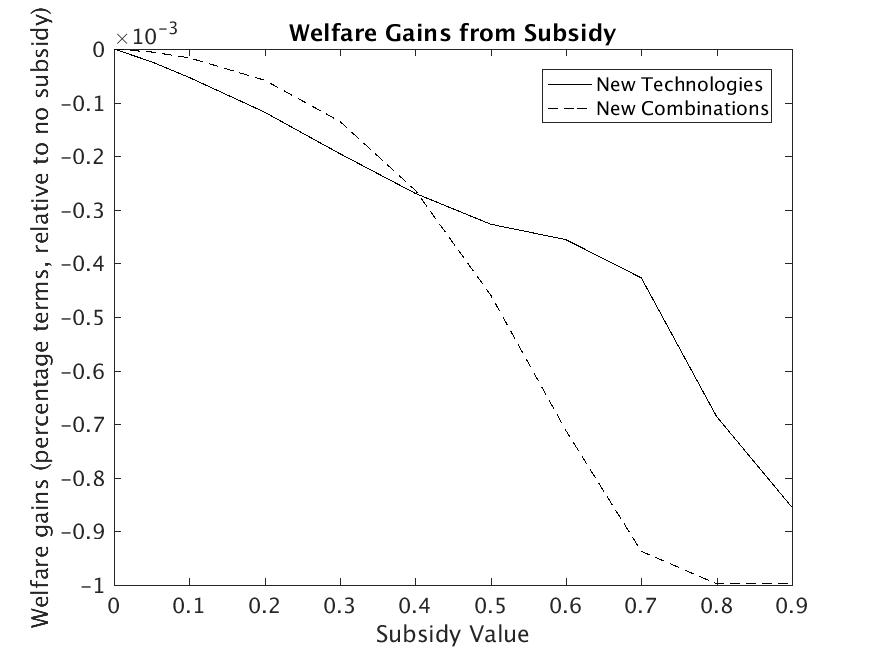
\includegraphics[width=.8\textwidth]{figures/10_years/welfare_gains.png}
\end{figure}
}

\frame{\frametitle{15 years of subsidy}
\begin{figure}[h!]
\centering
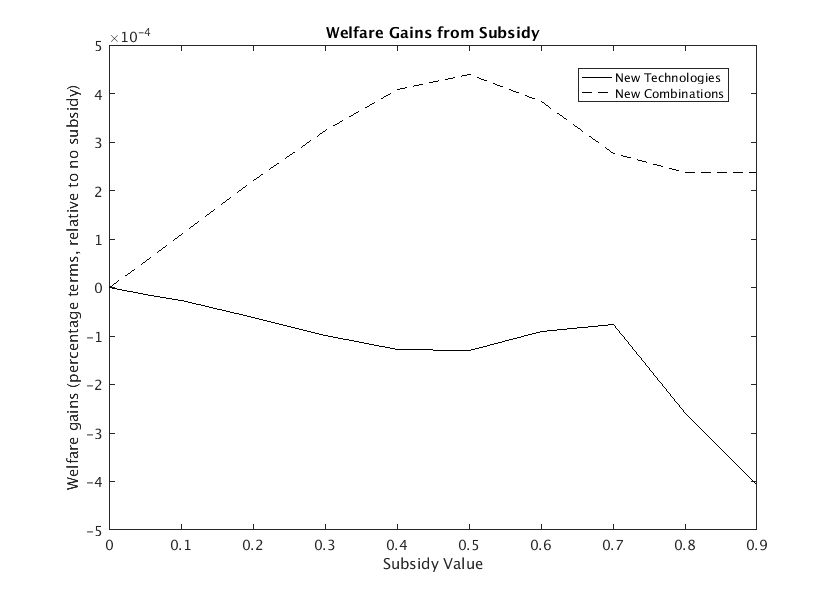
\includegraphics[width=.8\textwidth]{figures/15_years/welfare_gains.png}
\end{figure}
}

\frame{\frametitle{20 years of subsidy}
\begin{figure}[h!]
\centering
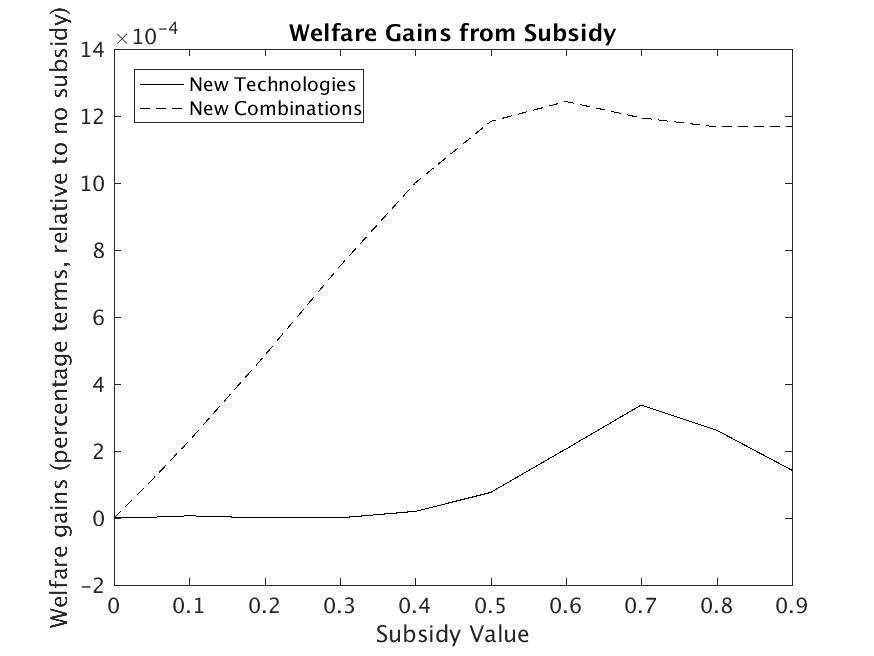
\includegraphics[width=.8\textwidth]{figures/20_years/welfare_gains.png}
\end{figure}
}

\frame{\frametitle{25 years of subsidy}
\begin{figure}[h!]
\centering
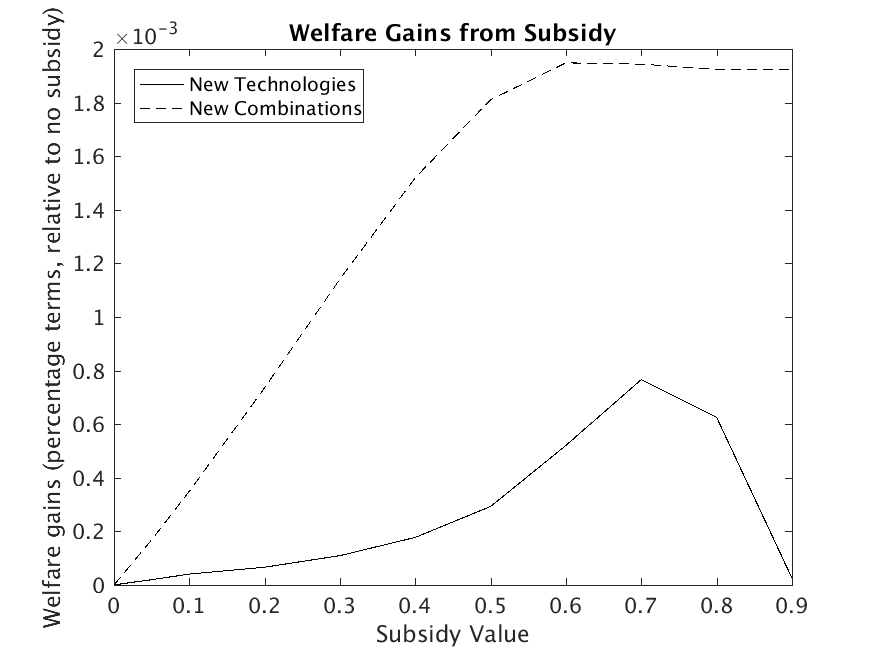
\includegraphics[width=.8\textwidth]{figures/25_years/welfare_gains.png}
\end{figure}
}

\title[Welfare Comparisons]{Economy with a 50\% Subsidy for 15 years}
\author[Alexandre Sollaci]{}
\institute[UChicago]{}
\date{}

\frame{
\titlepage
}

\begin{frame}\frametitle{Patent Shares}
\begin{figure}[h!]
\centering
\begin{subfigure}[b]{0.45\textwidth}
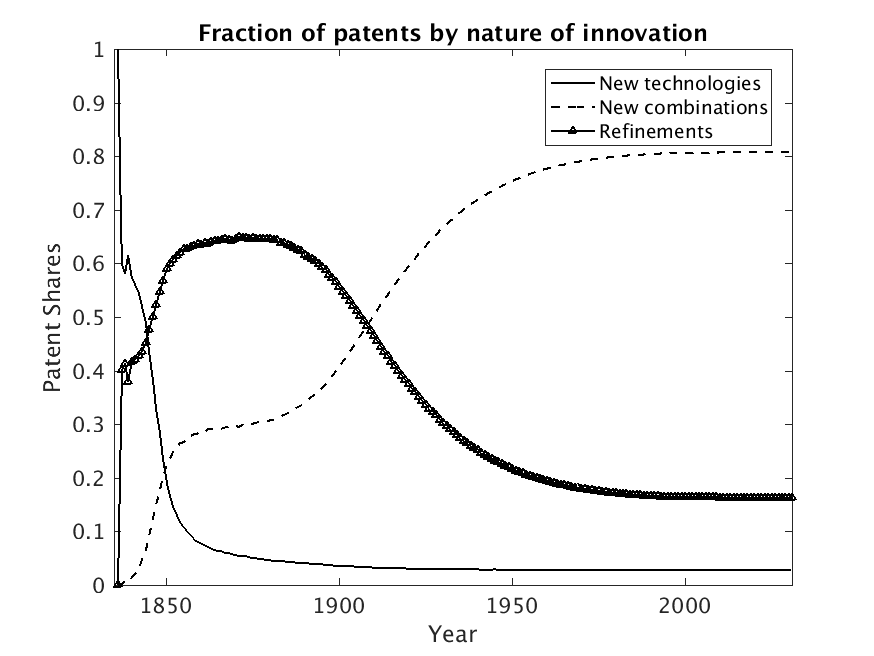
\includegraphics[width=\textwidth]{figures/15_years/patents.png}
\subcaption{Model.}
\end{subfigure}
\begin{subfigure}[b]{0.45\textwidth}
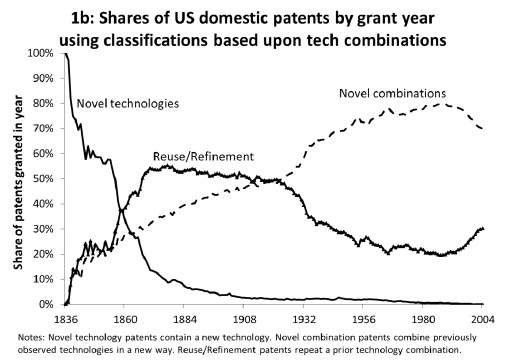
\includegraphics[width=\textwidth]{figures/patents_data.png}
\subcaption{Data.}
\end{subfigure}
\end{figure}
\end{frame}

\frame{\frametitle{Change in Share of Patents After Subsidy}
\begin{figure}[h!]
\centering
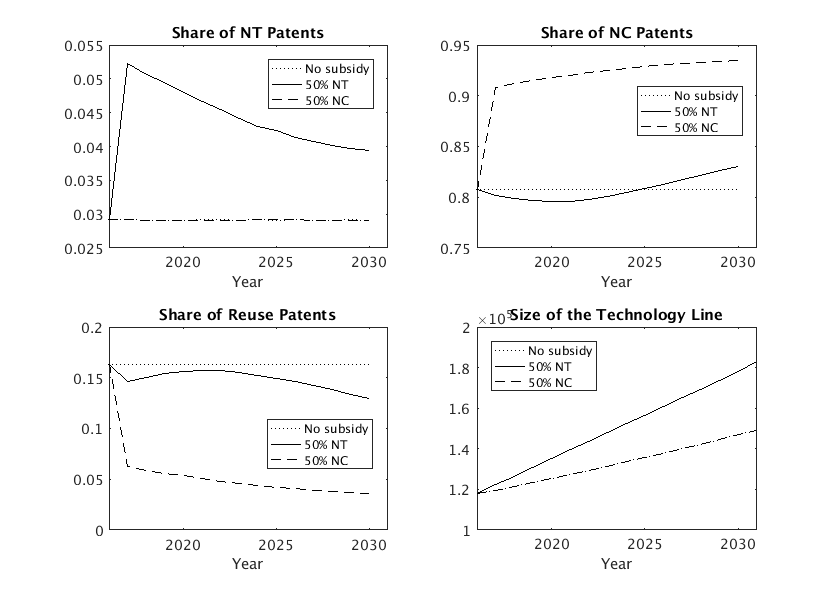
\includegraphics[width=.8\textwidth]{figures/15_years/patent_subs.png}
\end{figure}
}

\frame{\frametitle{Number of Patents Produced (does not change with subsidy)}
\begin{figure}[h!]
\centering
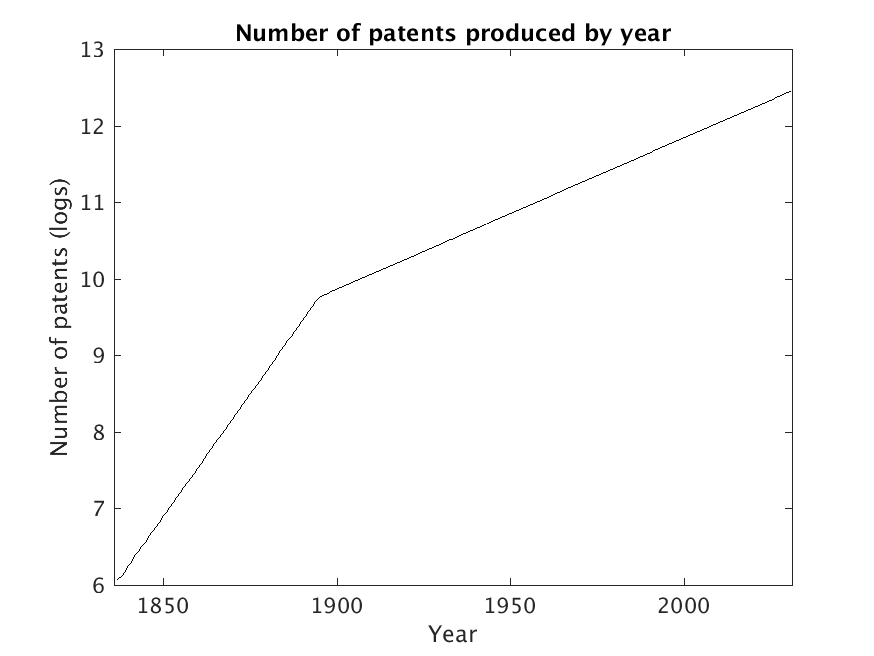
\includegraphics[width=.8\textwidth]{figures/15_years/num_pats.png}
\end{figure}
}

\frame{\frametitle{Aggregate Variables}
\begin{figure}[h!]
\centering
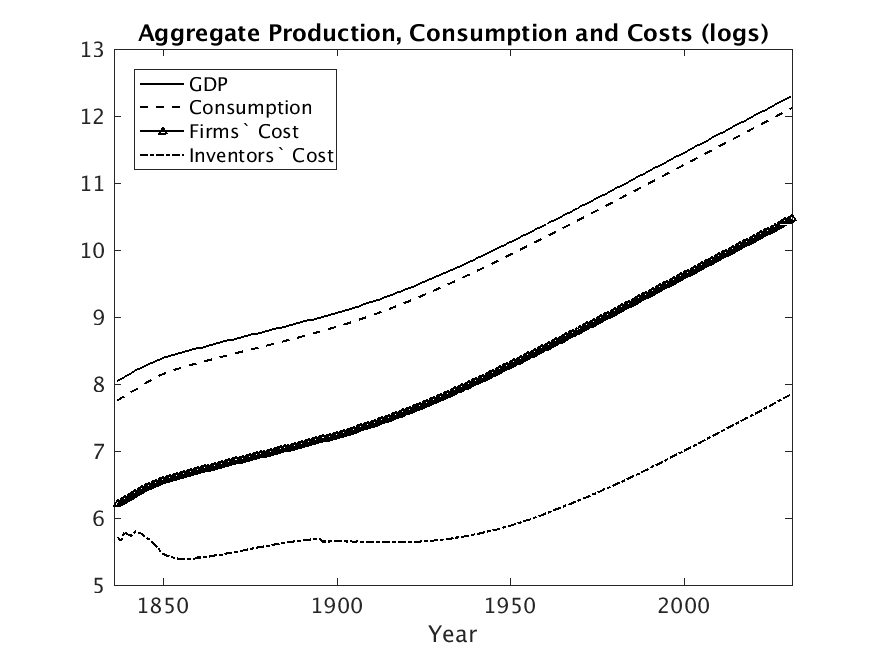
\includegraphics[width=.8\textwidth]{figures/15_years/aggregates.png}
\end{figure}
}

\frame{\frametitle{Aggregate Variables After Subsidy}
\begin{figure}[h!]
\centering
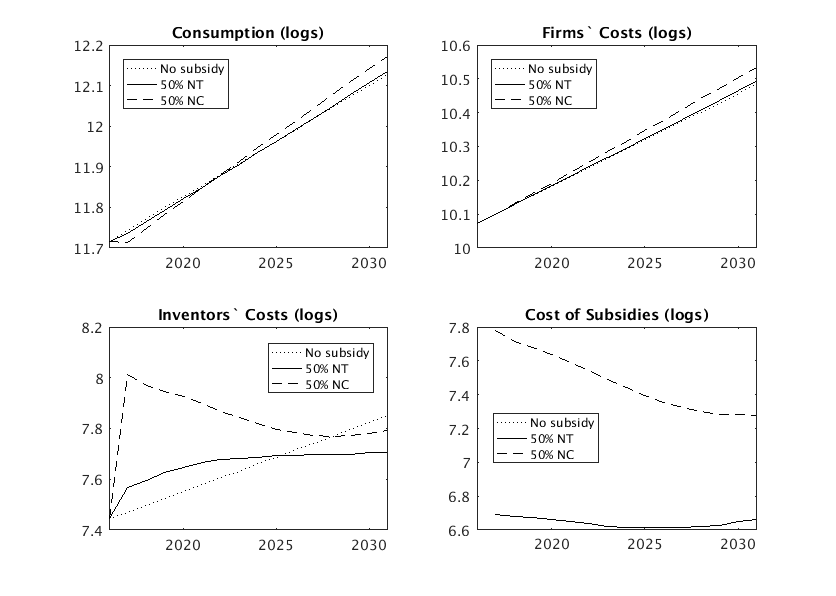
\includegraphics[width=.8\textwidth]{figures/15_years/aggregates_subs.png}
\end{figure}
}

\frame{\frametitle{Change in Aggregate Variables After Subsidy}
\begin{figure}[h!]
\centering
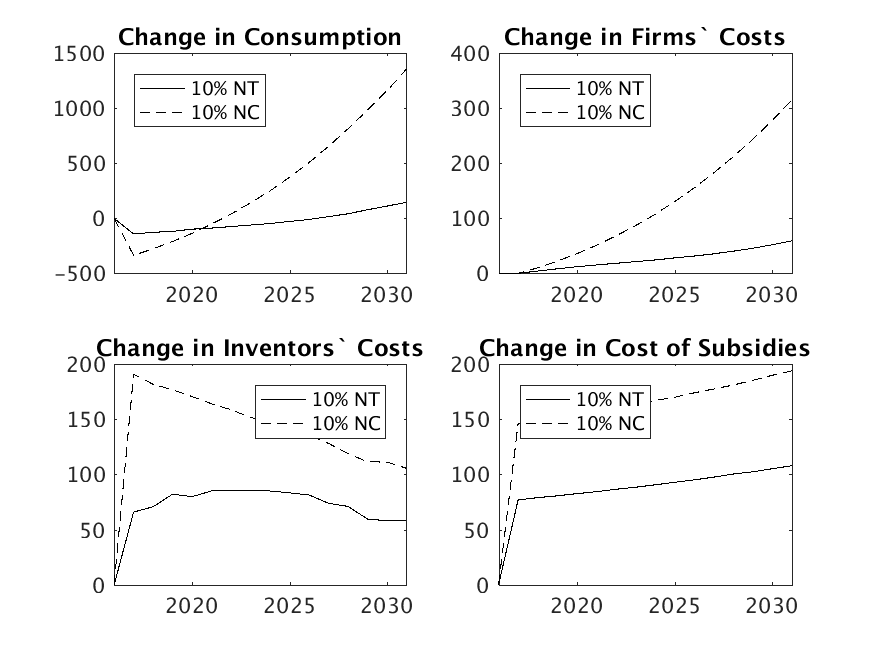
\includegraphics[width=.8\textwidth]{figures/15_years/change_aggregates_subs.png}
\end{figure}
}

\frame{\frametitle{GDP After Subsidy}
\begin{figure}[h!]
\centering
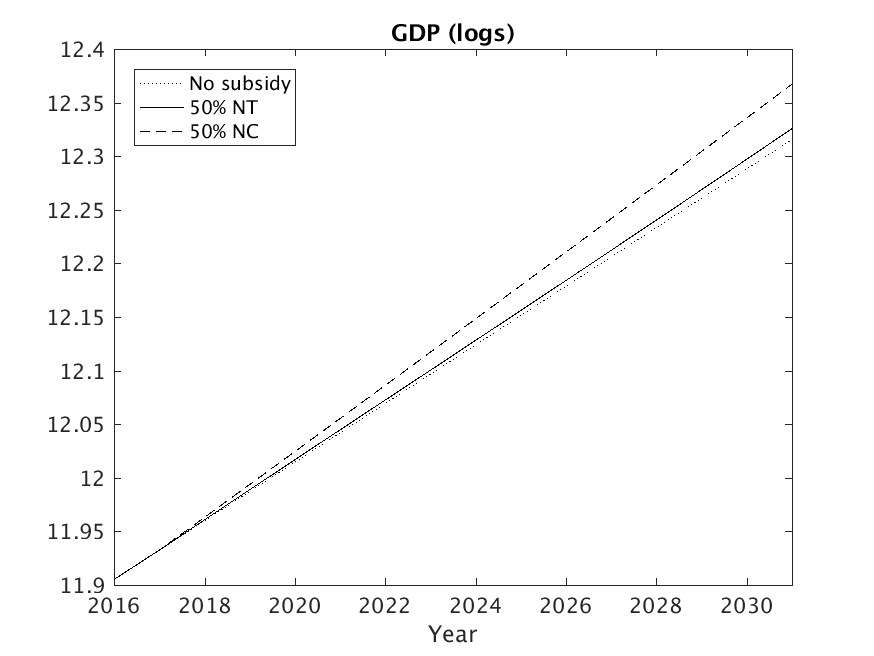
\includegraphics[width=.8\textwidth]{figures/15_years/GDP_subs.png}
\end{figure}
}

\frame{\frametitle{Growth Rate of Economy}
\begin{figure}[h!]
\centering
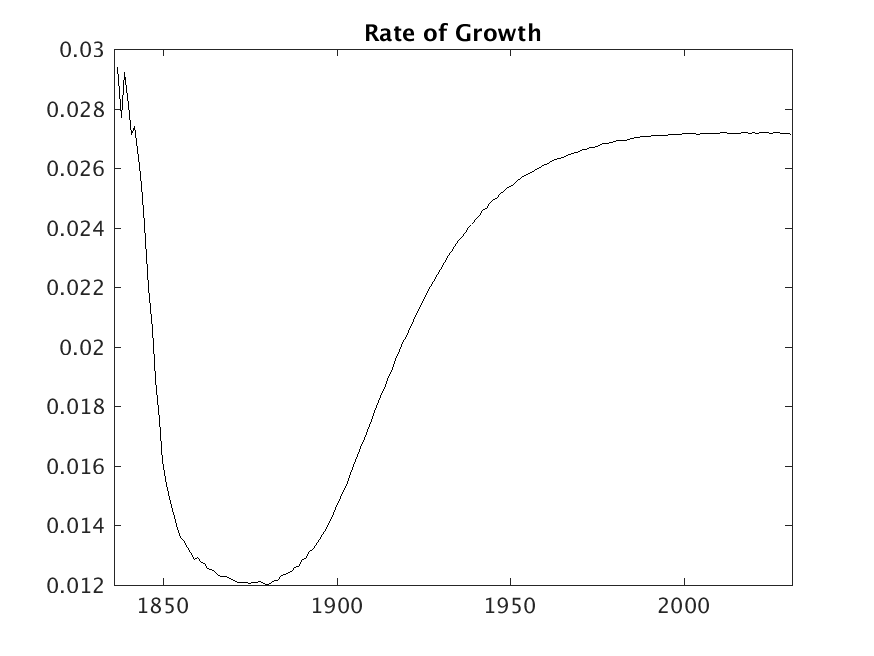
\includegraphics[width=.8\textwidth]{figures/15_years/growth.png}
\end{figure}
}

\frame{\frametitle{Growth Rate After Subsidy}
\begin{figure}[h!]
\centering
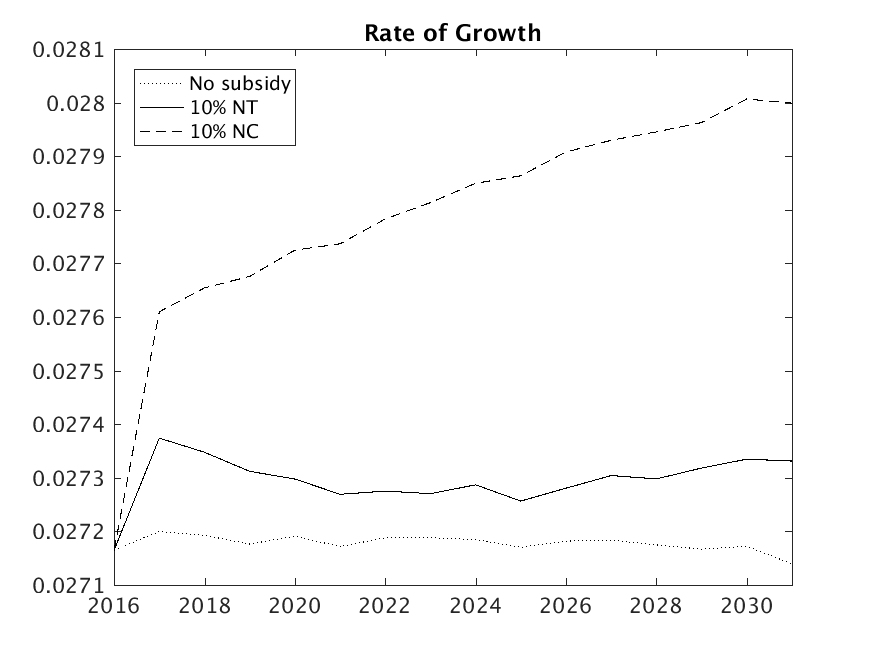
\includegraphics[width=.8\textwidth]{figures/15_years/growth_subs.png}
\end{figure}
}

\frame{\frametitle{Average Quality of Products in Economy After Subsidy}
\begin{figure}[h!]
\centering
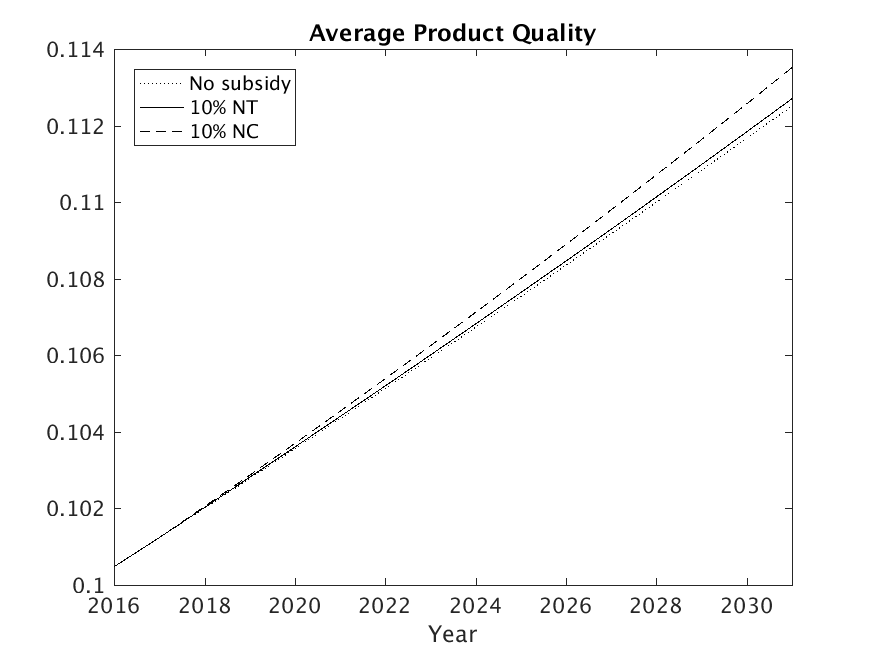
\includegraphics[width=.8\textwidth]{figures/15_years/quality_subs.png}
\end{figure}
}

\frame{\frametitle{Welfare Gains After Subsidy}
(This is the same figure as before)
\begin{figure}[h!]
\centering
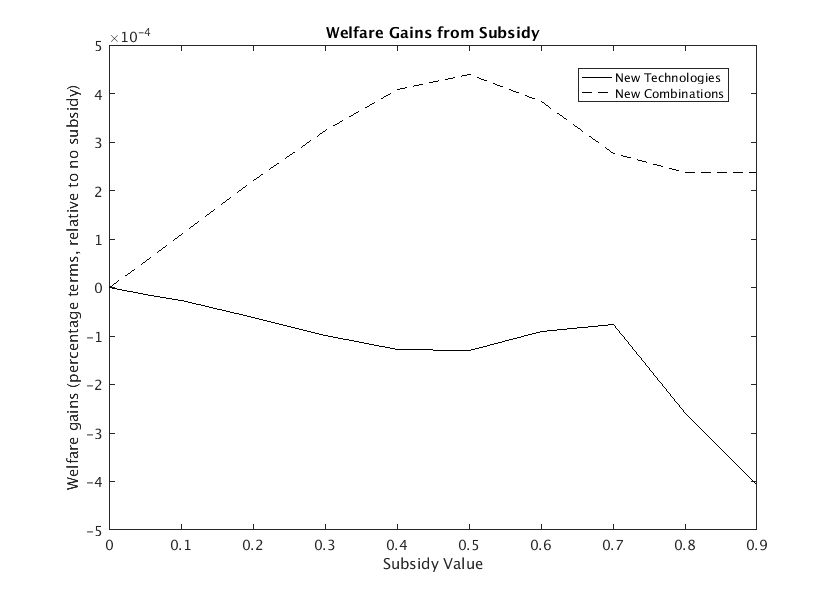
\includegraphics[width=.8\textwidth]{figures/15_years/welfare_gains.png}
\end{figure}
}

\end{document}